\chapter{Macrosegregation with incompressible fluid motion}
\begin{nolinkcolors} 
\minitoc
\end{nolinkcolors}
\newpage

this chapter discusses the following points:
\begin{itemize}
\item Review fluid mechanics briefly (MINI element and VMS and talk about the available solvers in Cimlib)
\item Give the VMS equations referring to Hachem article
\item Coupling the energy resolution from chapter 2 to fluid mechanics and solute balance
\item Make a transition to speak about freckles
\item Application: Ternary solidification with freckles
\item Application: Macroscopic Freckle prediction: pure FE
\item Application Multi-scale Freckle prediction: FE + grain structure (in which lies a part about nucleation-growth and how numerically 
		we reach a smaller scale, the scale of the grain boundaries)
\end{itemize}

\section{Introduction}
The previous chapter covered the energy solver ...

\section{Review fluid mechanics}
Review fluid mechanics briefly (MINI element and VMS and talk about the available solvers in Cimlib)

\section{VMS solver}
Give the VMS equations referring to Hachem article + weak form + stabilization

%taken from chapter 1
As for the last equation in \cref{tab:conservationeqs}, we follow the assumption of an incompressible liquid phase, which gives:
%---
\begin{align}
\label{eq:incompressiblity}
& \frac{\partial \r}{\partial t} = 0 
\end{align}

\section{Computational stability}
\subsection{CFL condition}
\subsection{Integration order}
Using P1 linear elements implies a P2 integration ? what are the advantages (time) and limitations ?




\section{Application to multicomponent alloys}

In chapter 2, we have shown that the efficiency of the temperature-based resolution resides in its performance when combined with 
thermodynamic tabulations. A multicomponent alloy consists of at least two solute elements, and 
therefore the tabulation size increases, hence the number of search operations also increases. 
To demonstrate the speed-up ability of the temperature-based approach while predicting all phase 
transformations during macrosegregation mainly caused by fluid flow, we consider the solidification of a ternary alloy, \tern{Fe}{2}{C}{30}{Cr}.
As illustrated in \cref{fig:mutlicomponent_geo}, the alloy domain has a cylinder shape close to 3-inch height $\times$ 1-inch diameter. 
Exact values are reported in \cref{table:data_case_ternary} with all material properties, initial and boundary conditions, 
as well as numerical parameters for the simulations. The melt steel is initially at \SI{1395}{\udegC}. The 
temperature of the bottom surface is imposed with a constant decreasing rate of \SI{0.1}{\uCR} starting 
with \SI{1380}{\udegC}, i.e. \SI{40}{\udegC} higher than the nominal liquidus temperature, as shown 
in \cref{fig:mutlicomponent_bc}. The other surfaces are kept adiabatic. The cylinder is held in a vertical position. 
In these conditions, and knowing that the carbon and chromium solutes have lightening effects on the liquid 
at nominal composition, the density inversion resulting from the composition gradient in the interdendritic 
liquid, may cause flow instability (segregation plumes) at the solidification front. While the selected alloy 
is a steel, this application is also representative of directional cooling in a single crystal casting, e.g. 
for nickel-base superalloys \citep{beckermann_development_2000}. \textbf{Figure 5c} also provides the 
transformation path of the alloy at nominal composition, i.e. assuming no macrosegregation and full 
thermodynamic equilibrium as computed with ThermoCalc and the TCFE6 database \citep{tcfe6_tcfe6:_2010, andersson_thermo-calc_2002}. 
A total of 5 phases need to be handled, the characteristic temperature for their formation being reported 
in \cref{fig:mutlicomponent_bc}.
%
\comment{Figure 5c: Computed transformation path \citep{tcfe6_tcfe6:_2010, andersson_thermo-calc_2002} at nominal composition
for the alloy \tern{Fe}{2}{C}{30}{Cr}.}
 %
\subsection{Tabulations}
\comment{update from last corrected version of the article}
Full thermodynamic equilibrium is considered in the present case. Due to macrosegregation, 
the average composition is expected to continuously vary in time and space during casting. 
Transformation paths are thus determined a priori for a set of average compositions around 
the nominal value. Hence, carbon content is arbitrarily varied in the interval [\SI{1.8}{\ucomposition}, \SI{2.2}{\ucomposition}] 
while chromium content variation is in the interval [\SI{27}{\ucomposition}, \SI{33}{\ucomposition}]. The offset of $\pm$ 10\%  with 
respect to the nominal composition value allows tabulating relatively small composition steps to 
ensure a good accuracy when compared to the corresponding ternary phase diagram. The average 
composition step is \SI{0.04}{\ucomposition} for carbon and \SI{0.6}{\ucomposition} for chromium, thus representing 2\% 
intervals with respect to the nominal composition. The temperature varies in the interval 
[\SI{100}{\udegC}, \SI{1600}{\udegC}] by \SI{5}{\udegC} steps. For each triplet (carbon content 
in \SI{}{\ucomposition} C, \textbf{HERE} , chromium content in \SI{}{\ucomposition} Cr, \textbf{HERE}, temperature in \si{\udegK}) 
corresponds a phase fraction $g^\phi$ and a pair of intrinsic phase composition (\textbf{HERE}). For the 5 
phases listed in \textbf{Figure 5c} (LIQ$\equiv$liquid, BCC$\equiv$ferrite, FCC$\equiv$austenite, 
$\text{M}_7 \text{C}_3 \equiv$carbide, CEM$\equiv$cementite), the enthalpy $h^\phi$ and density $\rho^\phi$, are tabulated 
as functions of temperature and phase intrinsic composition. If this latter input lies between two tabulated 
values, a linear interpolation is performed to determine the output, i.e. phase enthalpy and density. With 
the advancement of solidification, the liquid is enriched with solute by macrosegregation, which enables new 
solidification paths. It means that the primary solidifying phase is not necessarily the same as when considering 
the nominal composition. For this reason, the tabulation approach is interesting inasmuch as it provides phase 
transformation paths and values of phase properties that are compatible with the system’s actual composition. 
\textbf{Figure 6} summarizes the tabulated thermodynamic data for two sets of average composition for the considered 
ternary system. Note that in the present test case, phase densities are taken constant ($\rhos=\rhol=$ \SI{6725}{\udensity}). 
Therefore they are not tabulated. With this assumption, no shrinkage occurs upon phase change.
%
%-----------------
\begin{figure}[htbp]
\centering
   %------------
  \begin{subfigure}[t]{0.3\textwidth}
    \centering
	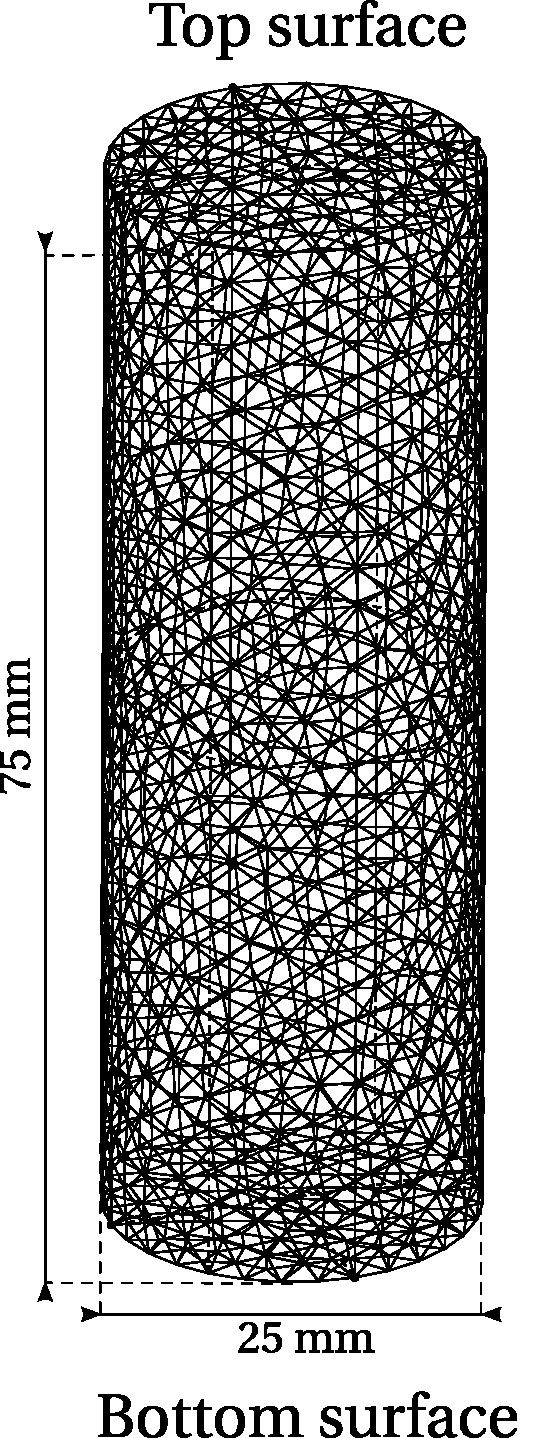
\includegraphics[height=6cm]{Chapter3/Graphics/multicomponent/Cylinder_nocolor_annotate.pdf}
	\caption{}
    \label{fig:mutlicomponent_geo}
  \end{subfigure}
   %------------
   \hspace{1mm}%\quad
   \begin{subfigure}[t]{0.5\textwidth}
    \centering
	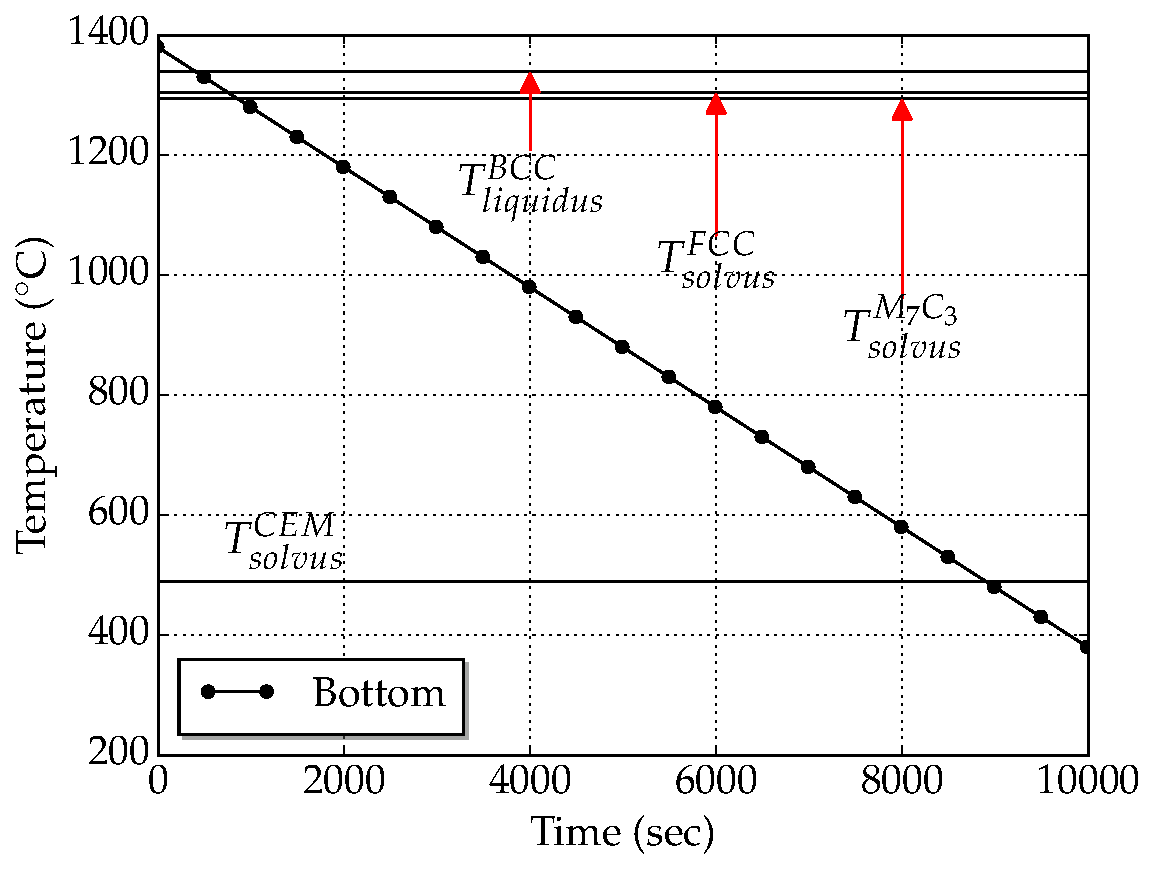
\includegraphics[height=6cm]{Chapter3/Graphics/multicomponent/BC.pdf}
	\caption{}
    \label{fig:mutlicomponent_bc}
  \end{subfigure}
  %------------------------------
\caption{Configurations for directional casting of (a) a 1 inch diameter $\times$ 3 inches height cylindrical domain for which
(b) temperature-time conditions are imposed at its bottom surface.} 
\label{fig:mutlicomponent_geobc}
\end{figure}
%-----------------
%
%----------------
\begin{tabulate}
%
% caption 
{Solidification parameters of the alloy \tern{Fe}{2}{C}{30}{Cr}.}
% label
{table:data_case_ternary}
% line separation (e.g. 1.5mm)
{0.8mm}
% column justification-number (e.g. |c|ll|)
{llll}
% header titles (should use the & sign to switch columns)
{\textbf{Parameter} & \textbf{Symbol} & \textbf{Value} & \textbf{Unit}}
% cells content (should use the & and // to switch columns and rows)
{
Nominal composition 			& $\wC_0$ 				& 2 					& \si{\ucomposition} 	\\ 
                    			& $\wCR_0$ 				& 30 					& \si{\ucomposition} 	\\ 
Characteristic temperatures 	& $T_\text{top},T_\text{bottom}$ 	& \textbf{FIGURE} & \si{\udegC} \\ 
Phase fraction 					& $g^\phi$ 				& Tabulations 	& $-$ 					\\ 
Phase enthalpy 					& $\h^\phi$ 			& Tabulations 	& $-$ 					\\ 
Phase composition 				& $\wC^\phi$ 			& Tabulations 	& \si{\ucomposition}  	\\ 
                   				& $\wCR^\phi$ 			& Tabulations 	& \si{\ucomposition}  	\\ 
Diffusion coefficients 			& $\avg{D_\text{C}}^l$ 	& \num{15e-10} 	& \si{\udiffusivity}  	\\ 
                        		& $\avg{D_\text{Cr}}^l$	 & \num{15e-10} 	& \si{\udiffusivity}  	\\ 
Dynamic viscosity  				& $\mul$ 					& \num{2e-3} 		& \si{\uviscosity}  	\\ 
Thermal expansion coefficient 	& \betaT 					& \num{8.96e-5} 	& \si{\ubetaT}  		\\ 
Solutal expansion coefficient 	& $\betawlC$ 				& \num{1.54e-3} 	& \si{\ubetawl}  		\\  
                              	& $\betawlCR$ 				& \num{1.72e-2} 	& \si{\ubetawl}  		\\ 
Thermal conductivity in the solid & $\ks$ 					& \num{40} 			& \si{\uconductivity}  	\\ 
Thermal conductivity in the liquid & $\kl$ 					& \num{28} 			& \si{\uconductivity}  	\\ 
Dendrite arm spacing 			& $\lambda$ 				& \num{60e-6} 	& \si{\metre}  			\\ 
Density 								& $\rref$ 			& \num{6725} 		& \si{\udensity}  		\\ 
\hline 
Initial temperature 	& $T_0$ & \num{1395}	& \si{\udegC}  \\ 
Ingot diameter 			&   	& \num{25e-3} 	& \si{\metre}  \\ 
Ingot length 			&   	& \num{75e-3} 	& \si{\metre}  \\ 
\hline 
FE mesh size 			&  		& \num{e-3} 	& \si{\metre}  \\ 
Time step 				& $\dt$ & \num{0.1} 	& \si{\second}  \\ 
Convergence criterion (residual) 	& $\varepsilon_R$ & \num{e-6} & $-$ \\ 
Convergence criterion (temperature) & $\varepsilon_T$ & \num{e-2} & \si{\udegK} 
}
%
\end{tabulate}
%-----------------
%
\section{Macroscopic freckle prediction}

\subsection{Introduction}
\comment{ I have shown the results of multicomponent alloy solidification, where we saw freckles. So let me do an introduction
about freckles, the need to prevent such defect from forming (superalloys, critical use in turbine blades}

\subsection{Experimental work}
\comment{ Then introduce the
experimental benchmark of Natalia and Sven from the article to show that there's an effort to understand, characterize and prevent 
if possible freckle formation. Show figures and some experimental results but quickly, no need to put many things and distract the reader }

\subsection{Macroscopic scale simulations}
\comment{ Introduce the FE model and algorithm then show pure FE RESULTS}
\subsubsection{Discussion}
In the literature, many successful attempts have been made to predict freckles since (for example CITE fellicelli, poireau) ... until coming to kohler thesis results in 2008. These authors tackled the problem from an qualitative perspective. To our knowledge, the only close-to-quantitative work in solidification literature was done by \citet{ramirez_evaluation_2003}, who attempted to draw a correlation (freckling criterion) between the process parameters and the occurence of freckles, (without any size or shape constraints, i.e. any flow instability that may appear and form the smallest freckle is considered). To accomplish this, they took a number of experiments done independently by \citet{pollock_breakdown_1996} and \citet{auburtin_freckle_2000} where the casting parameters vary one at a time: casting speed (R), thermal gradient (G), angle ($\theta$) with respect to vertical orientation and nominal composition ($\avg{w_0}$), giving a database for 6 different superalloys. The experimental results were compared to a modified Rayleigh number that accounts for the various parameters. It allowed them to define a threshold for freckle formation in Nickel-base superalloys, as well as Pb-Sn alloys.
\comment{ They have also investigated Pb-Sn alloys, check }
Other contributions by \citet{yuan_new_2012} and  \citet{karagadde_3-d_2014} used a medium scale model to compare the simulated formation of freckles with the results obtained by \citet{shevchenko_chimney_2013} (explain at bit more)
However, all simulations show common traits in their predictions: (some words about the freckle dimensions, shape, intensity). These properties do not exactly meet with the experimental observations, just like in the In-Ga experiment. We think that the hydrodynamics scale 
at which freckles are born, is much smaller than the FEM scale. Since the relevant physics are not solved, even the finest FE mesh will not
be enough to see the exact grain boundaries. (now it is time to do transition to CAFE)



\section{Meso-Macro freckle prediction}

parachute article :)
















